

\begin{document}

% Rectangular plate with torque arrows
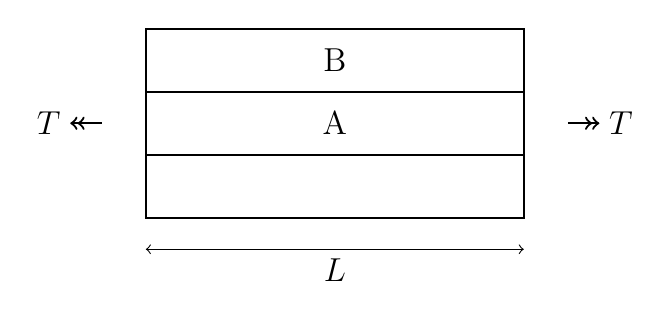
\begin{tikzpicture}[scale=0.8]
    % Plate outline
    \draw[thick] (0,0) rectangle (6,3);

    % Horizontal dividers
    \draw[thick] (0,1) -- (6,1);
    \draw[thick] (0,2) -- (6,2);

    % Layer labels
    \node at (3,0.5) {\large };
    \node at (3,1.5) {\large A};
    \node at (3,2.5) {\large B};

    % Horizontal dimension L
    \draw[<->] (0,-0.5) -- (6,-0.5);
    \node[below] at (3,-0.5) {\large $L$};

    % Torque arrows ←← on left
    \draw[<<-, thick] (-1.2,1.5) -- (-0.7,1.5);
    \node[left] at (-1.2,1.5) {\large $\boldsymbol{T}$};

    % Torque arrows →→ on right
    \draw[->>, thick] (6.7,1.5) -- (7.2,1.5);
    \node[right] at (7.2,1.5) {\large $\boldsymbol{T}$};
\end{tikzpicture}



% Concentric circular disc
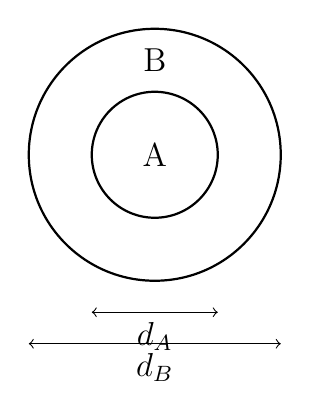
\begin{tikzpicture}[scale=0.8]
    % Outer and inner circles
    \draw[thick] (0,0) circle (2cm);  % Outer circle
    \draw[thick] (0,0) circle (1cm);  % Inner circle

    % Region labels
    \node at (0,0) {\large A};
    \node at (0,1.5) {\large B};

    % Diameter d_A
    \draw[<->] (-1,-2.5) -- (1,-2.5);
    \node[below] at (0,-2.5) {\large $d_A$};

    % Diameter d_B
    \draw[<->] (-2,-3) -- (2,-3);
    \node[below] at (0,-3) {\large $d_B$};
\end{tikzpicture}

\end{document}